\section{Exercises in appendix D}

\begin{prf}\label{sol_and}(Solution to~\ref{and})
 \begin{center}
  \begin{tabular}{|c|c||c|}\hline
        \,$P$\,    &    \,$Q$\,    &   \,$P \land Q$\,   \\
    \hline\hline
          $T$      &      $T$      &     $T$            \\
    \hline
          $T$      &      $F$      &     $F$            \\
    \hline
          $F$      &      $T$      &     $F$            \\
    \hline
          $F$      &      $F$      &     $F$            \\
    \hline
  \end{tabular}
 \end{center}
\end{prf}

\begin{prf}\label{sol_exer_ueq}(Solution to~\ref{exer_ueq})
First observe that the operation $\land$ is commutative and associative. (The former is
obvious and the latter may be easily checked by means of a truth table.)  Therefore if $A$,
$B$, and $C$ are propositions
\begin{align}\label{qref}
    A \land (B \land C) &\text{ iff }(A \land B)\land C \notag\\
                        &\text{ iff }  (B \land A) \land C \\
                        &\text{ iff }   B \land (A \land C). \notag
\end{align}
It then follows that
\begin{align*}
     (\exists x \in S)(\exists y \in T)\,P(x, y)
        &\text{ iff } (\exists x \in S)
            (\exists y) ((y \in T) \land P(x,y)) \\
        &\text{ iff } (\exists x)\bigl((x \in S) \land
            (\exists y) ((y \in T) \land P(x,y))\bigr) \\
        &\text{ iff } (\exists x)(\exists y)\bigl((x \in S)
             \land ((y \in T) \land P(x,y))\bigr) \\
        &\text{ iff } (\exists x)(\exists y)\bigl((y \in T)
             \land ((x \in S) \land P(x,y))\bigr)\quad
             \text{(by \eqref{qref})}\\
        &\text{ iff } (\exists y)(\exists x)\bigl((y \in T)
             \land ((x \in S) \land P(x,y))\bigr) \\
        &\text{ iff } (\exists y)\bigl((y \in T)
             \land (\exists x)((x \in S) \land P(x,y))\bigr) \\
        &\text{ iff } (\exists y)((y \in T)
             \land (\exists x \in S)\,P(x,y)) \\
        &\text{ iff } (\exists y \in T)(\exists x \in S)\,P(x,y) .
\end{align*}
Notice that at the third and sixth steps we used the remark made in the last paragraph of
section~\ref{d_and_c}.
\end{prf}

\begin{prf}\label{sol_equiv_impl}(Solution to~\ref{equiv_impl})
 \begin{center}
  \begin{tabular}{|c|c||c|c|c|}\hline
           (1)     &     (2)       &        (3)               &    (4)        &      (5)                \\
        \,$P$\,    &    \,$Q$\,    &   \,$P \Rightarrow Q$\,  & \,$\sim P$\,  &  \,$Q \lor (\sim P)$\,  \\
    \hline\hline
          $T$      &      $T$      &     $T$                  &   $F$         &    $T$                  \\
    \hline
          $T$      &      $F$      &     $F$                  &   $F$         &    $F$                  \\
    \hline
          $F$      &      $T$      &     $T$                  &   $T$         &    $T$                  \\
    \hline
          $F$      &      $F$      &     $T$                  &   $T$         &    $T$                  \\
    \hline
  \end{tabular}
 \end{center}
The third and fifth columns have the same truth values.
\end{prf}




%END Appendix d












\section{Exercises in appendix F}
 \nopagebreak
\begin{prf}\label{sol_uoveri_fin}(Solution to~\ref{uoveri_fin})
If $S$, $T$, and $U$ are sets, then
 \begin{align*}
    x \in S \cup (T \cap U) \quad
         &\text{iff} \quad x \in S \text{ or } x \in T \cap U \\
         &\text{iff} \quad x \in S  \text{ or }
                  (x \in T  \text{ and } x \in U) \\
         &\text{iff} \quad (x \in S \text{ or }  x \in T)
                  \text{ and } (x \in S \text{ or } x \in U) \\
         &\text{iff} \quad  x  \in  S \cup T
                  \text{ and } x  \in  S \cup U \\
         &\text{iff} \quad  x  \in  (S \cup T) \cap (S \cup U).
 \end{align*}
Problem~\ref{prob_disj_conj} was used to get the third line.
\end{prf}

\begin{prf}\label{sol_uoveri_inf}(Solution to~\ref{uoveri_inf})
If $T$ is a set and $\sfml S$ is a family of sets, then
 \begin{align*}
   x \in T \cup \bigl(\bigcap\sfml S\bigr) \quad
       &\text{iff} \quad x \in T \text{ or } x \in \bigcap\sfml S \\
       &\text{iff} \quad x \in T \text{ or }
              (\forall S \in \sfml S)\, x \in S \\
       &\text{iff} \quad (\forall S \in \sfml S)(x \in T
               \text{ or } x \in S) \\
       &\text{iff} \quad (\forall S \in \sfml S)\, x \in T \cup S \\
       &\text{iff} \quad x \in \bigcap\{T \cup S\colon S \in \sfml S\}.
 \end{align*}
To obtain the third line we used the principle mentioned in the last paragraph of
section~\ref{d_and_c} of appendix~\ref{log_con}.
\end{prf}

\begin{prf}\label{sol_prop_compl_union}(Solution to~\ref{prop_compl_union})
Here is one proof: A necessary and sufficient condition for an element $x$ to belong to the
complement of $S \cup T$ is that it not belong to $S$ or to~$T$. This is the equivalent to its
belonging to both $S^c$ and~$T^c$, that is, to the intersection of the complements of $S$
and~$T$.

A second more ``formalistic'' proof looks like this :
 \begin{align*}
   x \in (S \cup T)^c  \quad
             &\text{iff} \quad  x \notin S \cup T \\
             &\text{iff} \quad  \sim(x \in S \cup T) \\
             &\text{iff} \quad  \sim(x \in S \text{ or }
                                       x \in T) \\
             &\text{iff} \quad  \sim(x \in S) \text{ and }
                                       \sim(x \in T) \\
             &\text{iff} \quad  x \notin S \text{ and }
                                       x \notin T \\
             &\text{iff} \quad  x \in S^c \text{ and }
                                       x \in T^c \\
             &\text{iff} \quad  x \in S^c \cap T^c.
 \end{align*}
This second proof is not entirely without merit: at each step only one definition or fact is
used.  (For example, the result presented in example~\ref{exam_demorg1} justifies the fourth
``iff''.)  But on balance most readers, unless they are very unfamiliar with the material,
would probably prefer the first version.  After all, it's easier to read English than to
translate code.
\end{prf}

\begin{prf}\label{sol_comp_of_union}(Solution to~\ref{comp_of_union})
 \nopagebreak
Here is another formalistic proof.  It is a good idea to try and rewrite it in
ordinary English.
 \begin{align*}
    x  \in  (\bigcup \sfml S)^c  \quad
      &\text{iff} \quad  x \notin \bigcup \sfml S  \\
      &\text{iff} \quad  \sim (x \in \bigcup \sfml S) \\
      &\text{iff} \quad  \sim(\exists S \in \sfml S)(x \in S) \\
      &\text{iff} \quad  (\forall S \in \sfml S)\sim (x \in S) \\
      &\text{iff} \quad  (\forall S \in \sfml S)(x \notin S) \\
      &\text{iff} \quad  (\forall S \in \sfml S)(x \in S^c) \\
      &\text{iff} \quad  x \in \bigcap\{S^c\colon S \in \sfml S\}. \qedhere
 \end{align*}
\end{prf}

\begin{prf}\label{sol_prop_decomp_union}(Solution to~\ref{prop_decomp_union})
To see that  $S \setminus T$ and $T$ are disjoint, notice that
  \begin{align*}
     (S \setminus T) \cap T  &= S \cap T^c \cap T  \\
                             &= S \cap \emptyset  \\
                             &= \emptyset.
  \end{align*}
Furthermore,
  \begin{align*}
     (S \setminus T) \cup T  &=  (S \cap T^c ) \cup T \\
                             &=  (S \cup T) \cap (T^c \cup T) \\
                             &=  S \cup T.
  \end{align*}
As usual $S$ and $T$ are regarded as belonging to some universal set, say $U$. Then $T^c \cup
T$ is all of $U$ and its intersection with $S \cup T$ (which is contained in $U$) is just $S \cup T$.
\end{prf}

\begin{prf}\label{sol_exer_diff_union}(Solution to~\ref{exer_diff_union})
We know from proposition~\ref{prop_union_sets} (e) that $S \cup T  =  S$ if and only if $T
\subseteq S$.  But proposition~\ref{prop_decomp_union} tells us that $S \cup T = (S \setminus
T) \cup T$.  Thus $(S \setminus T) \cup T  =  S$ if and only if $T \subseteq S$.
\end{prf}





%END Appendix F














\section{Exercises in appendix G}

\begin{prf}\label{sol_2x_is_x}(Solution to~\ref{2x_is_x})
If $x + x = x$, then
\begin{align*} x &= x + 0 \\
                 &= x + (x + (-x)) \\
                 &= (x + x) + (-x) \\
                 &= x + (-x) \\
                 &= 0.       \qedhere
\end{align*}
\end{prf}

\begin{prf}\label{sol_arith_exer1}(Solution to~\ref{arith_exer1})
Use associativity and commutativity of addition.
  \begin{align*}
     (w + x) + (y + z)  &= ((w + x) + y) + z \\
                        &= (w + (x + y)) + z \\
                        &= ((x + y) + w) + z \\
                        &= z + ((x + y) + w) \\
                        &= z + (x + (y + w)).
  \end{align*}
The first, second, and last equalities use associativity of addition; steps 3 and 4 use its
commutativity.
\end{prf}






%END appendix G













\section{Exercises in appendix H}

\begin{prf}\label{sol_pos}(Solution to~\ref{pos})
By definition $x > 0$ holds if and only if $0 < x$, and this holds (again by definition) if
and only if $x - 0 \in \Po$. Since $-0 = 0$ (which is obvious from $0 + 0 = 0$ and the fact
that the additive identity is unique), we conclude that $x > 0$ if and only if
  \[ x = x + 0 = x + (-0) = x - 0 \in \Po\,.   \qedhere \]
\end{prf}

\begin{prf}\label{sol_mult_pos}(Solution to~\ref{mult_pos})
By the preceding exercise $x > 0$ implies that $x \in \Po$; and $y < z$ implies $z - y \in
\Po$. Since $\Po$ is closed under multiplication, $x(z - y)$ belongs to $\Po$. Thus
  \begin{align*}
       xz - xy  &= xz + (-(xy)) \\
                &= xz + x(-y) \qquad\text{ by problem~\ref{arith_prob1}} \\
                &= x(z + (-y)) \\
                &= x(z - y) \in \Po\,.
  \end{align*}
This shows that $xy < xz$.
\end{prf}

\begin{prf}\label{sol_mult_ineq}(Solution to~\ref{mult_ineq})
Since $0 < w < x$ and $y > 0$, we may infer from exercise \ref{mult_pos} that $yw < yx$.
Similarly, we obtain $xy < xz$ from the conditions $0 < y < z$ and $x > 0$ (which holds by the
transitivity of $<$, proposition~\ref{lt_tran}). Then
  \[ wy = yw < yx = xy < xz\,. \]
Thus the desired inequality $wy < xz$ follows (again by transitivity of~$<$).
\end{prf}







%END appendix H















\section{Exercises in appendix I}

\begin{prf}\label{sol_prop_intrs_ind}(Solution to~\ref{prop_intrs_ind})
Since $1$ belongs to $A$ for every $A \in \sfml A$, it is clear that $1 \in \cap\sfml A$.
If $x \in \cap\sfml A$, then $x \in A$ for every $A \in \sfml A$. Since each set $A$ in
$\sfml A$ is inductive, $x + 1 \in A$ for every $A \in \sfml A$.  That is, $x + 1 \in
\cap\sfml A$.
\end{prf}

\begin{prf}\label{sol_exer_mi1}(Solution to~\ref{exer_mi1})
Let $S$ be the set of all natural numbers for which the assertion is true.  Certainly $1$
belongs to $S$.  If $n \in S$, then $\sum_{k=1}^n k = \frac12 n(n + 1)$.  Therefore
 \begin{align*}
     \sum_{k=1}^{n+1}k &= \biggl(\sum_{k=1}^n k\biggr) + (n+1) \\
                       &= \frac12 n(n + 1) + (n + 1)           \\
                       &= \frac12(n + 1)(n + 2),
 \end{align*}
which shows that $n + 1 \in S$.  Thus $S$ is an inductive subset of $\N$.  We conclude from
corollary~\ref{cor_mi2} that $S = \N$. In other words, the assertion holds for all $n \in \N$.
\end{prf}

\begin{prf}\label{sol_prop_well_ord}(Solution to~\ref{prop_well_ord})
Let $K$ be a subset of $\N$ which has no smallest member.  We show $K = \emptyset$.  Let
  \[ J = \{n \in \N \colon n < k \text{ for all } k \in K\}\,. \]
Certainly $1$ belongs to~$J$.  [If not, there would exist $c \in K$ such that $1 \ge c$.  From
proposition~\ref{prop_natno_pos} we see that $c = 1$.  Thus $1$ belongs to $K$ and is the
smallest member of $K$, contrary to our assumption.]

Now suppose that $n \in J$ and prove that $n + 1 \in J$. If $n + 1 \notin J$, then there
exists $k \in K$ such that $n + 1 \ge k$.  By the inductive hypothesis $n < k$.  Thus $n < k
\le n + 1$.  We conclude from problem~\ref{prob_less_pos}(b) that $k = n + 1$. But, since $n$
is smaller than every member of $K$, this implies that $n + 1$ is the smallest member of $K$.
But $K$ has no smallest member.  Therefore we conclude that $n + 1 \in J$.

We have shown that $J$ is an inductive subset of $\N$.  Then $J = \N$ (by
theorem~\ref{thm_mth_ind}).  If $K$ contains any element at all, say $j$, then $j \in J$; so
in particular $j < j$. Since this is not possible, we conclude that $K = \emptyset$.
\end{prf}







%END of appendix I























\section{Exercises in appendix J}

\begin{prf}\label{sol_exer_sup1}(Solution to~\ref{exer_sup1})

(a) A number $x$ belongs to the set $A$ if $x^2 - 4x + 3 < 3$; that is, if $x(x - 4) < 0$.
This occurs if and only if  $x > 0$ and $x < 4$.  Thus $A = (0,4)$; so $\sup A = 4$ and $\inf
A = 0$.

(b) Use beginning calculus to see that $f'(x) = 2x - 4$. Conclude that the function $f$ is
decreasing on the interval $(-\infty,2)$ and is increasing on $(2, 3)$. Thus $f$ assumes a
minimum at $x = 2$. Since $f(2) = -1$, we see that $B = [-1,\infty)$.  Thus $\sup B$ does not
exist and $\inf B = -1$.
\end{prf}

\begin{prf}\label{sol_prop_sup_prod}(Solution to~\ref{prop_sup_prod})
As in the hint let $\ell = \sup A$ and  $m = \sup B$, and suppose that $\ell$, $m > 0$. If $x
\in AB$, then there exist $a \in A$ and $b \in B$ such that $x = ab$.  From $a \le \ell$ and
$b \le m$ it is clear that $x \le \ell m$; so $\ell m$ is an upper bound for $AB$.

Since $AB$ is bounded above it must have a least upper bound, say~$c$.  Clearly $c \le \ell
m$; we show that $\ell m \le c$. Assume, to the contrary, that $c < \ell m$. Let $\epsilon =
\ell m - c$.  Since $\epsilon > 0$ and $\ell$ is the least upper bound for $A$ we may choose
an element $a$ of $A$ such that $a > \ell - \epsilon(2m)^{-1}$.  Similarly, we may choose $b
\in B$ so that $b > m - \epsilon(2\ell)^{-1}$. Then
  \begin{align*}
     ab &> \bigl(\ell - \epsilon(2m)^{-1}\bigr)\bigl(m - \epsilon(2\ell)^{-1}\bigr) \\
        &= \ell m - \epsilon + \epsilon^2(4\ell m)^{-1} \\
        &> \ell m - \epsilon \\
        &= c.
  \end{align*}
This is a contradiction, since $ab$ belongs to $AB$ and $c$ is an upper bound of $AB$.  We
have shown
  \[ \sup(AB) = c = \ell m = (\sup A)(\sup B) \]
as required.
\end{prf}

\begin{rem}  It is not particularly difficult to follow the details of the preceding proof.
But that is \emph{not} the same thing as \emph{understanding} the proof!  It is easy to see,
for example, that \emph{if} we choose $a > \ell - \epsilon(2m)^{-1}$ and $b > m -
\epsilon(2\ell)^{-1}$, \emph{then} $ab>c$.   But that still leaves room to be puzzled.  You
might reasonably say when shown this proof, ``Well, that certainly \emph{is} a proof.  And it
looks very clever.  But what I don't understand is how did you know to choose $a$ and $b$ in
just that particular (or should I say `peculiar'?) way?  Do you operate by fits of
inspiration, or a crystal ball, or divination of entrails, or what?''  The question deserves
an answer. Once we have assumed $c$ to be an upper bound smaller than $\ell m$ (and set
$\epsilon = \ell m - c$), our hope is to choose $a \in A$ close to $\ell$ and $b \in B$ close
to $m$ in such a way that their product $ab$ exceeds $c$.  It is difficult to say immediately
\emph{how} close $a$ should be to $\ell$ (and $b$ to $m$).  Let's just say that $a > \ell -
\delta_1$ and $b > m - \delta_2$, where $\delta_1$ and $\delta_2$ are small positive numbers.
We will figure out \emph{how} small they should be in a moment. Then
  \[ ab > (\ell - \delta_1)(m - \delta_2) = \ell m - m\delta_1
                                       - \ell\delta_2 + \delta_1\delta_2\,. \]
Since $\delta_1\delta_2$ is positive, we can simplify the preceding inequality and write
  \begin{equation}\label{eqn1_sup_prod}
           ab > \ell m - m\delta_1 - \ell\delta_2\,.
  \end{equation}
What we \emph{want} to get at the end of our computation is
  \begin{equation}\label{eqn2_sup_prod}
           ab > c = \ell m - \epsilon.
  \end{equation}
Now comparing what we have \eqref{eqn1_sup_prod} with what we want \eqref{eqn2_sup_prod}, we
see that all we need to do is choose $\delta_1$ and $\delta_2$ in such a way that
  \begin{equation}\label{eqn3_sup_prod}
             m\delta_1 + \ell\delta_2 < \epsilon
  \end{equation}
(for then $\ell m - (m\delta_1 + \ell\delta_2) > \ell m - \epsilon = c$, and we are done).  To
guarantee that the sum of two numbers is less than $\epsilon$ it suffices to choose both of
them to be less than $\epsilon/2$.  Clearly, we have $m\delta_1 < \epsilon/2$ if we choose
$\delta_1 < \epsilon(2m)^{-1}$; and we have $\ell\delta_2 < \epsilon/2$ if we choose $\delta_2
< \epsilon(2\ell)^{-1}$.  And that's all we need.
\end{rem}

\begin{prf}\label{sol_prop_exist_sqrt}(Solution to~\ref{prop_exist_sqrt})
Let $A = \{t > 0 \colon t^2 < a\}$. The set $A$ is not empty since it contains $a(1 +
a)^{-1}$. [$a^2(1 + a)^{-2} < a(1 + a)^{-1} < a$.]  It is easy to see that $A$ is bounded
above by $M := \max\{1,a\}$.  [If $t \in A$ and $t \le 1$, then $t \le M$; on the other hand,
if $t \in A$ and $t > 1$, then $t < t^2 < a \le M$.]  By the \emph{least upper bound axiom}
(\ref{axiom_lub}) $A$ has a supremum, say $x$. It follows from the \emph{axiom of trichotomy}
(\ref{axiom_trichot}) that exactly one of three things must be true: $x^2 < a$, $x^2 > a$, or
$x^2 = a$.  We show that $x^2 = a$ by eliminating the first two alternatives.

First assume that $x^2 < a$.  Choose $\epsilon$ in $(0,1)$ so that $\epsilon < 3^{-1}x^{-2}(a
- x^2)$. Then
  \begin{align}\label{eqn1_sqrt}
       (1 + \epsilon)^2 &= 1 + 2\epsilon + \epsilon^2 \\
                        &< 1 + 3\epsilon
  \end{align}
so that
  \[ x^2(1 + \epsilon)^2 < x^2(1 + 3\epsilon) < a\,. \]
Thus $x(1 + \epsilon)$ belongs to $A$. But this is impossible since $x(1 + \epsilon) > x$ and
$x$ is the supremum of $A$.

Now assume $x^2 > a$. Choose $\epsilon$ in $(0,1)$ so that $\epsilon < (3a)^{-1}(x^2 - a)$.
Then by \eqref{eqn1_sqrt}
  \begin{equation}\label{eqn2_sqrt}
        a < x^2(1 + 3\epsilon)^{-1} < x^2(1 + \epsilon)^{-2}\,.
  \end{equation}
Now since $x = \sup A$ and $x(1 + \epsilon)^{-1} < x$, there must exist $t \in A$ such that
$x(1 + \epsilon)^{-1} < t < x$. But then
  \[ x^2(1 + \epsilon)^{-2} < t^2 < a\,, \]
which contradicts~\eqref{eqn2_sqrt}. Thus we have demonstrated the existence of a number $x
\ge 0$ such that $x^2 = a$.  That there is only one such number has already been proved: see
problem~\ref{prob_sqrt_uniq}.
\end{prf}






%END appendix J





















\section{Exercises in appendix K}

\begin{prf}\label{sol_lex1}(Solution to~\ref{lex1})
Suppose that $(x,y) = (u,v)$. Then
 \[\bigl\{\{x,y\},\{x\}\bigr\} = \bigl\{\{u,v\},\{u\}\bigr\}.\]
We consider two cases.

Case 1: \quad $\{x,y\} = \{u,v\}$ and $\{x\} = \{u\}$.  The second equality implies that $x =
u$.  Then from the first equality we infer that $y = v$.

Case 2: \quad $\{x,y\} = \{u\}$ and $\{x\} = \{u,v\}$.  We derive $x = u = y$ from the first
equality and $u = x = v$ from the second.  Thus $x = y = u = v$. In either case $x = u$ and $y = v$.
The converse is obvious.
\end{prf}

\begin{prf}\label{sol_lex2}(Solution to~\ref{lex2})

(a) $f(\frac12) = 3$;

(b) Notice that $(1 - x)^{-1}$ does not exist if $x = 1$, $(1 + (1 - x)^{-1})^{-1}$
does not exist if $x = 2$, and $(1 - 2(1 + (1 - x)^{-1})^{-1})^{-1}$ does not exist if $x =
0$; so $\dom f = \R \setminus \{0,1,2\}$.  \qedhere
\end{prf}

\begin{prf}\label{sol_lex3}(Solution to~\ref{lex3})
We can take the square root of $g(x) = -x^2 - 4x - 1$ only when $g(x) \ge 0$, and since we
take its reciprocal, it should not be zero.  But $g(x) > 0$ if and only if $x^2 + 4 x + 1 < 0$
if and only if $(x + 2)^2 < 3$ if and only if $\abs{x + 2} < \sqrt3$ if and only if $-2 -
\sqrt3 < x < -2 + \sqrt3$.  So $\dom f = (-2 - \sqrt3, -2 + \sqrt3)$.
\end{prf}





%END appendix K

















\section{Exercises in appendix L}

\begin{prf}\label{sol_exer_fcn1}(Solution to~\ref{exer_fcn1})
We may write $A$ as the union of three intervals
 \[ A = (-4,4) = (-4,-2) \cup [-2,1) \cup [1,4)\,. \]
Then
 \begin{equation}\label{exer_fcn1_eqn1}
%  \begin{aligned}
     f^{\sto}(A) = f^{\sto}\bigl(\,(-4,4)\,\bigr)\\
                 = f^{\sto}\bigl(\,(-4,-2)\,\bigr) \cup f^{\sto}\bigl(\,[-2,1)\,\bigr)
                           \cup f^{\sto}\bigl(\,[1,4)\,\bigr)\,.
%  \end{aligned}
 \end{equation}
(This step is justified in the next section by \ref{prop_f_union}.) Since $f$ is constant on
the interval $(-4,-2)$ we see that $f^{\sto}\bigl(\,(-4,-2)\,\bigr) = \{-1\}$.  On the
interval $[-2,1)$ the function increases from $f(-2) = 3$ to $f(0) = 7$ and then decreases to
$f(1) = 6$ so that $f^{\sto}\bigl(\,[-2,1)\,\bigr) = [3,7]$.  (This interval is closed because
both $-2$ and $0$ belong to~$[-2,1)$.) Finally, since $f$ is decreasing on $[1,4)$ we see that
$f^{\sto}\bigl(\,[1,4)\,\bigr) = \bigl(f(4),f(1)\,\bigr] = (\frac14,1]$.  Thus from equation
\eqref{exer_fcn1_eqn1} we conclude that
     \[f^{\sto}(A) = \{-1\} \cup (\tfrac14,1] \cup [3,7]. \qedhere \]
\end{prf}

\begin{prf}\label{sol_exer_fcn2}(Solution to~\ref{exer_fcn2})
Use techniques from beginning calculus. The function is a fourth degree polynomial, so $f(x)
\sto \infty$ as $x \sto -\infty$ and as $x \sto \infty$.  Thus the range of $f$ is not bounded
above. The minimum value of the range will occur at a critical point, that is, at a point
where $f'(x) = 0$.  But this occurs at $x = -3$, $x = 0$, and $x = 2$. The values of $f$ at
these points are, respectively $-188$, $0$, and $-63$.  We conclude that $\ran f = [-188,\infty)$.
\end{prf}

\begin{prf}\label{sol_exer_fcn3}(Solution to~\ref{exer_fcn3})
Notice that the arctangent function is strictly increasing (its derivative at each $x$ is $(1
+ x^2)^{-1}$).  Its range is $(-\pi/2,\pi/2)$.  Thus $f^{\gets}(B) =
f^{\gets}\bigl((\pi/4,2)\bigr) = f^{\gets}\bigl((\pi/4,\pi/2)\bigr) = (1, \infty)$.
\end{prf}

\begin{prf}\label{sol_exer_fcn4}(Solution to~\ref{exer_fcn4})
For $-\sqrt{9 - x^2}$ to lie between $1$ and $3$, we would need $-3 < \sqrt{9 - x^2} < -1$.
But since the square root function on $\R$ takes on only positive values, this is not
possible.  So $f^{\gets}(B) = \emptyset$.
\end{prf}

\begin{prf}\label{sol_exer_fcn5}(Solution to~\ref{exer_fcn5})
For $x \le \frac13$, $f(x) \le 1$ which implies $g(f(x)) = -1$. For $x \in (\frac13,1)$, $f(x)
\in (1,3)$, so $g(f(x)) = 9x^2$. For $1 \le x \le 2$, $f(x) = 2$, so $g(f(x)) = -1$.  Finally,
for $x > 2$, $f(x) = 2$ and therefore $g(f(x)) = 4$.
 \begin{figure}[!h]
    \[ \scalebox{.40}{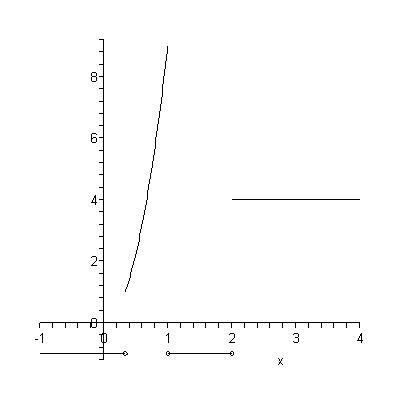
\includegraphics{zzzgraph}} \qedhere \]
 \end{figure}
\end{prf}

\begin{prf}\label{sol_prop_assoc_comp}(Solution to~\ref{prop_assoc_comp})
Associativity: for every $x$
 \[ (h \circ (g \circ f))(x) = h((g \circ f)(x)) = h(g(f(x)))=
              (h \circ g)(f(x)) = ((h \circ g) \circ f)(x)\,; \]
so $h \circ (g \circ f) = (h \circ g) \circ f$.

To see that composition is not commutative take, for example, $f(x) = x + 1$ and $g(x) = x^2$.
Since $(g \circ f)(1) = 4$ and $(f \circ g)(1) = 2$, the functions $g \circ f$ and $f \circ g$
cannot be equal.
\end{prf}






%END appendix L



















\section{Exercises in appendix M}

\begin{prf}\label{sol_exam_inj_fcn}(Solution to~\ref{exam_inj_fcn})
If $f(x) = f(y)$, then $(x + 2)(3y - 5) = (y + 2)(3x - 5)$. Thus $6y - 5x = 6x - 5y$, which
implies $x = y$.
\end{prf}

\begin{prf}\label{sol_exer_inj_q}(Solution to~\ref{exer_inj_q})
Suppose that $m$ and $n$ are positive integers with no common prime factors. Let $f\bigl(\frac
mn\bigr) = 2^m3^n$. Then  $f$ is injective by the \emph{unique factorization theorem} (see,
for example, \cite{BirkhoffMacL:1953}, page~21).
\end{prf}

\begin{prf}\label{sol_exer_surj}(Solution to~\ref{exer_surj})
Let $f(x) = \frac1x - 1$ for $x \ne 0$ and $f(0)~=~3$.
\end{prf}

\begin{prf}\label{sol_exer_bij1}(Solution to~\ref{exer_bij1})
Define $f\colon \Z \sto \N$ by
    \[f(n) = \begin{cases} 2n + 1, &\text{for $n \ge 0$} \\
                             -2n,  &\text{for $n < 0$}.
             \end{cases}   \qedhere \]
\end{prf}

\begin{prf}\label{sol_exer_bij2}(Solution to~\ref{exer_bij2})
Define $f\colon \R \sto (0,1)$ by $f(x) = \frac12 + \frac1\pi \arctan x$.
\end{prf}

\begin{prf}\label{sol_exer_bij3}(Solution to~\ref{exer_bij3})
Let $\Sp^1$ be $\{(x,y)\colon  x^2 + y^2 = 1\}$.  Define $f\colon [0,1) \sto \Sp^1$ by $f(t) =
(\cos(2\pi t), \sin (2\pi t))$.
\end{prf}

\begin{prf}\label{sol_exer_bij4}(Solution to~\ref{exer_bij4})
Let
   \[g(x) = \begin{cases}   3 - 2x,   &\text{for $0 \le x < 1$} \\
                          f(x),       &\text{for $1 \le x \le 2$}\\
                        \frac12(3-x), &\text{for $2 < x \le 3$}.
            \end{cases}   \qedhere\]
\end{prf}

\begin{prf}\label{sol_exer_bij5}(Solution to~\ref{exer_bij5})
$\bigl[-\frac\pi2, \frac\pi2\bigr]$.
\end{prf}

\begin{prf}\label{sol_prop_f_finv}(Solution to~\ref{prop_f_finv})

(a) We show that if $y \in f^{\sto}(f^\gets(B))$, then $y \in B$.  Suppose that $y \in
f^{\sto}(f^\gets(B))$. Then (by the definition of $f^{\sto}$) there exists $x \in f^\gets(B)$
such that $y = f(x)$. From $x \in f^\gets(B)$ we infer (using the definition of $f^\gets$)
that $f(x) \in B$. That is, $y \in B$.

(b) Let $f(x) = x^2$ and $B = \{-1\}$. Then $f^{\sto}(f^\gets(B)) = f^{\sto}(f^\gets\{-1\}) =
f^{\sto}(\emptyset) = \emptyset \ne~B$.

(c) Suppose that $f$ is surjective. Show that $ B \subseteq f^{\sto}(f^\gets(B))$ by showing
that $y \in B$ implies $y \in f^{\sto}(f^\gets(B))$.  If $y \in B$, then (since $f$ is
surjective) there exists $x \in S$ such that $y = f(x)$. Since $f(x) \in B$, we see that $x
\in f^\gets(B)$ (by the definition of $f^\gets$).  From this it follows (using the definition
of $f^{\sto}$) that $y = f(x) \in f^{\sto}(f^\gets(B))$. \qedhere
\end{prf}

\begin{prf}\label{sol_prop_f_union}(Solution to~\ref{prop_f_union})
This requires nothing other than the definitions of $\cup$ and $f^{\sto}$:
 \begin{align*}
   y \in f^{\sto}(A \cup B)
   &\text{ iff there exists $x \in A \cup B$ such that $y=f(x)$}\\
   &\text{ iff there exists $x \in A$ such that $y = f(x)$ or} \\
   &\qquad\text{ there exists $x \in B$ such that $y = f(x)$} \\
   &\text{ iff $y \in f^{\sto}(A)$ or $y \in f^{\sto}(B)$} \\
   &\text{ iff $y \in f^{\sto}(A) \cup f^{\sto}(B)$.}  \qedhere
   \end{align*}
\end{prf}

\begin{prf}\label{sol_prop_finv_intrs}(Solution to~\ref{prop_finv_intrs})
Here the definitions of $\cap$ and $f^\gets$ are used:
\begin{align*}
   x \in f^\gets(C \cap D)
   &\text{ iff $f(x) \in C \cap D$} \\
   &\text{ iff $f(x) \in C$ and $f(x) \in D$} \\
   &\text{ iff $x \in f^\gets(C)$ and $x \in f^\gets(D)$} \\
   &\text{ iff $x \in f^\gets(C) \cap f^\gets(D)$.}  \qedhere
\end{align*}
\end{prf}

\begin{prf}\label{sol_prop_f_fam}(Solution to~\ref{prop_f_fam})

(a) Show that if $y \in f^{\sto}(\bigcap \sfml A)$, then $y \in \bigcap\{f^{\sto}(A)
\colon A \in \sfml A\}$.  Suppose that $y \in f^{\sto}(\bigcap \sfml A)$. Then there
exists $x \in \bigcap\sfml A$ such that $y = f(x)$. Since $x$ belongs to the intersection
of the family $\sfml A$ it must belong to every member of $\sfml A$. That is, $x \in A$
for every $A \in \sfml A$. Thus $y = f(x)$ belongs to $f^{\sto}(A)$ for every $A \in
\sfml A$; and so $y \in \bigcap\{f^{\sto}(A)\colon A \in \sfml A\}$.

(b) Suppose $f$ is injective. If $y \in \bigcap\{f^{\sto}(A)\colon A \in \sfml A\}$, then
$y \in f^{\sto}(A)$ for every $A \in \sfml A$. Choose a set $A_0 \in \sfml A$. Since $y
\in f^{\sto}(A_0)$, there exists $x_0 \in A_0$ such that $y = f(x_0)$. The point $x_0$
belongs to every member of $\sfml A$. To see this, let $A$ be an arbitrary set belonging
to $\sfml A$. Since $y \in f^{\sto}(A)$, there exists $x \in A$ such that $y = f(x)$; and
since $f(x) = y = f(x_0)$ and $f$ is injective, we conclude that $x_0 = x \in A$. Thus we
have shown that $x_0 \in \bigcap\sfml A$ and therefore that $y = f(x_0) \in
f^{\sto}(\bigcap\sfml A)$.

(c) If $y \in f^{\sto}(\bigcup\sfml A)$, then there exists $x \in \bigcup\sfml A$ such
that $y = f(x)$. Since $x \in \bigcup\sfml A$ there exists $A \in \sfml A$ such that $x
\in A$. Then $y = f(x) \in f^{\sto}(A)$ and so $y \in \bigcup\{f^{\sto}(A): A \in \sfml
A\}$. Conversely, if $y$ belongs to $\bigcup\{f^{\sto}(A): A \in \sfml A\}$, then it must
be a member of $f^{\sto}(A)$ for some $A \in \sfml A$. Then $y = f(x)$ for some $x \in A
\subseteq \bigcup\sfml A$ and therefore $y = f(x) \in f^{\sto}(\bigcup\sfml A)$. \qedhere
\end{prf}



\begin{prf}\label{sol_prop_finv_unique}(Solution to~\ref{prop_finv_unique})
Let $f\colon S \sto T$ and suppose that $g$ and $h$ are inverses of $f$. Then
  \[ g = g \circ I_T = g \circ (f \circ h) = (g \circ f) \circ h = I_S
                 \circ h = h\,.\qedhere \]
\end{prf}

\begin{prf}\label{sol_exer_inv_trig}(Solution to~\ref{exer_inv_trig})
\emph{Arcsine} is the inverse of the restriction of the \emph{sine} function to the interval
$[-\frac\pi2,\frac\pi2]$.  The \emph{arccosine} is the inverse of the restriction of
\emph{cosine} to $[0,\pi]$.  And \emph{arctangent} is the inverse of the restriction of
\emph{tangent} to $(-\frac\pi2,\frac\pi2)$.
\end{prf}

\begin{prf}\label{sol_prop_rinv_surj}(Solution to~\ref{prop_rinv_surj})
Suppose that $f$ has a right inverse~$f_r$. For each $y \in T$ it is clear that $y = I_T(y) =
f\bigl(f_r(y)\bigr) \in \ran f$; so $\ran f = T$ and $f$ is surjective.

Conversely, suppose that $f$ is surjective. Then for every $y \in T$ the set
$f^{\gets}(\{y\})$ is nonempty. For each $y \in T$ let $x_y$ be a member of $f^{\gets}(\{y\})$
and define
 \[ f_r\colon T \sto S\colon y \mapsto x_y\,. \]
Then $f\bigl(f_r(y)\bigr) = f(x_y) = y$, showing that $f_r$ is a right inverse of~$f$.
(The reader who has studied a bit of set theory will likely have noticed the unadvertised
use of the
 \index{axiom!of choice}%
 \index{choice, axiom of}%
\emph{axiom of choice} in this proof. It is used in this fashion throughout the text.)
\end{prf}






%END appendix M
















\section{Exercises in appendix N}

\begin{prf}\label{sol_prod_exer}(Solution to~\ref{prod_exer})
The existence of the function has already been demonstrated: if $f = (f^1,f^2)$, then $(\pi_k
\circ f)(t) = \pi_k\bigl(f^1(t),f^2(t)\bigr) = f^k(t)$ for $k = 1,2$ and $t \in T$.

To prove uniqueness suppose that there is a function $g \in \fml F(T,S_1 \times S_2)$ such
that $\pi_k \circ g = f^k$ for $k = 1,2$. Then $g(t) = \bigl(\pi_1(g(t)), \pi_2(g(t))\bigr) =
\bigl(f^1(t),f^2(t)\bigr) = \bigl(f^1,f^2\bigr)(t)$ for $k = 1,2$ and $t \in T$.  So $g =
\bigl(f^1,f^2\bigr)$.
\end{prf}





%END appendix N




















\section{Exercises in appendix O}

\begin{prf}\label{sol_prop_card_n}(Solution to~\ref{prop_card_n})
We wish to demonstrate that for all natural numbers $m$ and $n$ if there is a bijection from
$\{1,\dots, m\}$ onto $\{1,\dots, n\}$, then $m = n$.  To accomplish this use induction
on~$n$.

First, suppose that for an arbitrary natural number $m$ we have $\{1,\dots, m\} \sim \{1\}$.
That is, we suppose that there exists a bijection $f$ from $\{1, \dots, m\}$ onto $\{1\}$.
Then since $f(1) = 1 = f(m)$ and $f$ is injective, we conclude that $m = 1$. This establishes
the proposition in the case $n = 1$.

Next, we assume the truth of the result for some particular $n \in \N$: for every $m \in \N$
if $\{1,\dots, m\} \sim \{1,\dots, n\}$, then $m = n$.  This is our inductive hypothesis. What
we wish to show is that for an arbitrary natural number $m$ if $\{1,\dots, m\} \sim \{1,\dots,
n+1\}$, then $m = n+1$.  Suppose then that $m \in \N$ and $\{1,\dots, m\} \sim
\{1,\dots,n+1\}$. Then there is a bijection $f$ from $\{1,\dots,m\}$ onto $\{1,\dots,n + 1\}$.
Let $k = f^{-1}(n + 1)$. The restriction of $f$ to the set $\{1,\dots,k - 1,k~+~1~, \dots,m\}$
is a bijection from that set onto $\{1,\dots,n\}$. Thus
  \begin{equation}\label{eqn_card_n1}
         \{1,\dots,k - 1,k + 1,\dots,m\} \sim \{1,\dots,n\}.
  \end{equation}
Furthermore, it is easy to see that
  \begin{equation}\label{eqn_card_n2}
         \{1,\dots,m - 1\} \sim \{1,\dots,k - 1,k + 1,\dots,m\}.
  \end{equation}
(The required bijection is defined by $g(j) = j$ if $1 \le j \le k - 1$ and $g(j) = j + 1$ if
$k \le j \le m - 1$.) From \eqref{eqn_card_n1}, \eqref{eqn_card_n2}, and
proposition~\ref{prop_ce_er} we conclude that
  \[ \{1,\dots,m-1\} \sim \{1,\dots,n\}\,. \]
By our inductive hypothesis, $m - 1 = n$. This yields the desired conclusion $m = n + 1$.
\end{prf}

\begin{prf}\label{sol_prop_card_union}(Solution to~\ref{prop_card_union})
The result is trivial if $S$ or $T$ is empty; so we suppose they are not. Let $m = \card S$
and $n = \card T$.  Then $S \sim \{1,\dots,m\}$ and $T \sim \{1,\dots,n\}$. It is clear that
  \[ \{1,\dots,n\} \sim \{m+1,\dots,m + n\}\,. \]
(Use the map $j \mapsto j + m$ for $1 \le j \le n$.)  Thus $T \sim \{m + 1,\dots,m + n\}$. Let
$f \colon S \sto \{1,\dots,m\}$ and $g \colon T \sto \{m + 1,\dots,m + n\}$ be bijections.
Define $h \colon S \cup T \sto \{1,\dots,m + n\}$ by
  \[h(x) = \begin{cases}
              f(x), &\text{for $x \in S$}\\
              g(x), &\text{for $x \in T$.}
           \end{cases} \]
Then clearly $h$ is a bijection.  So $S \cup T$ is finite and $\card(S \cup T) = m + n = \card S + \card T$.
\end{prf}

\begin{prf}\label{sol_lem_card_sub}(Solution to~\ref{lem_card_sub})
Proceed by mathematical induction. If $C \subseteq \{1\}$, then either $C = \emptyset$, in
which case $\card C = 0$, or else $C = \{1\}$, in which case $\card C = 1$. Thus the lemma is
true if $n = 1$.

Suppose then that the lemma holds for some particular $n \in \N$. We prove its correctness for
$n + 1$. So we assume that $C \subseteq \{1,\dots,n + 1\}$ and prove that $C$ is finite and
that $\card C \le n + 1$.  It is clear that $C \setminus \{n + 1\} \subseteq \{1,\dots,n\}$.
By the inductive hypothesis $C \setminus \{n + 1\}$ is finite and $\card(C \setminus \{n +
1\}) \le n$.  There are two possibilities: $n + 1 \notin C$ and $n + 1 \in C$. In case $n + 1$
does not belong to $C$, then $C = C \setminus \{n + 1\}$; so $C$ is finite and $\card C \le n
< n + 1$.  In the other case, where $n + 1$ does belong to $C$, it is clear that $C$ is finite
(because $C \setminus \{n + 1\}$ is) and we have (by proposition~\ref{prop_card_union})
  \begin{align*}
       \card C  &= \card\bigl((C \setminus \{n + 1\}) \cup \{n + 1\}\bigr) \\
                &= \card(C \setminus \{n + 1\}) + \card(\{n + 1\}) \\
                &\le n + 1.        \qedhere
  \end{align*}
\end{prf}

\begin{prf}\label{sol_prop_ce_sub}(Solution to~\ref{prop_ce_sub})
Suppose that $S$ is infinite.  We prove that there exists a proper subset $T$ of $S$ and a
bijection $f$ from $S$ onto $T$. We choose a sequence of distinct elements $a_k$ in $S$, one
for each $k \in \N$. Let $a_1$ be an arbitrary member of $S$. Then $S \setminus \{a_1\} \ne
\emptyset$. (Otherwise $S \sim \{a_1\}$ and $S$ is finite.) Choose $a_2 \in S \setminus
\{a_1\}$. Then $S \setminus \{a_1,a_2\} \ne \emptyset$. (Otherwise $S \sim \{a_1,a_2\}$ and
$S$ is finite.) In general, if distinct elements $a_1,\dots,a_n$ have been chosen, then $S
\setminus \{a_1,\dots,a_n\}$ cannot be empty; so we may choose $a_{n+1} \in S \setminus
\{a_1,\dots,a_n\}$. Let $T = S \setminus \{a_1\}$, and define $f \colon S \sto T$ by
   \[f(x) = \begin{cases}
                 a_{k+1}, &\text{if $x=a_k$ for some $k$}\\
                 x,       &\text{otherwise}.
            \end{cases}\]
Then $f$ is a bijection from $S$ onto the proper subset $T$ of~$S$.

For the converse construct a proof by contradiction. Suppose that $S \sim T$ for some proper
subset $T \subseteq S$, and assume further that $S$ is finite, so that $S \sim \{1,\dots,n\}$
for some $n \in \N$. Then by proposition \ref{prop_card_sub} the set $S \setminus T$ is finite
and, since it is nonempty, is therefore cardinally equivalent to $\{1,\dots,p\}$ for some $p
\in \N$. Thus
  \begin{align*}
       n &= \card S\\
         &= \card T\\
         &= \card (S \setminus (S \setminus T))\\
         &= \card S - \card(S \setminus T)\qquad \text{(by problem \ref{prob_card_diff})} \\
         &= n - p.
  \end{align*}
Therefore $p = 0$, which contradicts the earlier assertion that $p \in \N$.
\end{prf}

\begin{prf}\label{sol_exer_int_inf}(Solution to~\ref{exer_int_inf})
The map $x \mapsto \frac12x$ is a bijection from the interval $(0,1)$ onto the interval
$(0,\frac12)$, which is a proper subset of~$(0,1)$.
\end{prf}

\begin{prf}\label{sol_prop_ran_fin}(Solution to~\ref{prop_ran_fin})
Since $f$ is surjective it has a right inverse $f_r$ (see proposition \ref{prop_rinv_surj}).
This right inverse is injective, since it has a left inverse (see
proposition~\ref{prop_linv_inj}). Let $A = \ran f_r$. The function $f_r$ establishes a
bijection between $T$ and~$A$. Thus $T \sim A \subseteq S$. If $S$ is finite, so is $A$ (by
proposition \ref{prop_card_sub}) and therefore so is $T$.
\end{prf}

\begin{prf}\label{sol_prop_preimg_fin}(Solution to~\ref{prop_preimg_fin})
Let $B = \ran f$. Then $S \sim B \subseteq T$. If $T$ is finite, so is $B$ (by
proposition~\ref{prop_card_sub}) and therefore so is~$S$.
\end{prf}





%END appendix O















\section{Exercises in appendix P}

\begin{prf}\label{sol_prop_sub_cntbl}(Solution to~\ref{prop_sub_cntbl})
If $S$ is finite there is nothing to prove; so we suppose that $S$ is an infinite subset of
$T$.  Then $T$ is countably infinite.  Let $f \colon \N \sto T$ be an enumeration of the
members of $T$. The restriction of $f$ to the set $f^\gets(S) \subseteq \N$ is a bijection
between $f^\gets(S)$ and $S$; so we may conclude that $S$ is countable provided we can prove
that $f^\gets(S)$ is. Therefore it suffices to show that \emph{every} subset of $\N$  is
countable.

Let $A$ be an infinite subset of $\N$. Define inductively elements $a_1 < a_2 < \dots$ in $A$.
(Let $a_1$ be the smallest member of $A$. Having chosen $a_1 < a_2 < \dots < a_n$ in $A$,
notice that the set $A \setminus \{a_1,\dots,a_n\}$ is not empty and choose $a_{n+1}$ to be
the smallest element of that set.)  Let $a \colon \N \sto A$ be the function $n \mapsto a_n$.
It is clear that $a_k \ge k$ for all $k$ and, since $a_k < a_{k+1}$ for all $k$, that $a$ is
injective.  To see that $a$ is surjective, assume that it is not and derive a contradiction.
If $a$ is not surjective, then the range of $a$ is a proper subset of $A$.  Let $p$ be the
smallest element of $A \setminus \ran a$.  Since $p \in A \setminus \ran a \subseteq A
\setminus \{a_1,\dots,a_p\}$, we see from the definition of $a_{p+1}$ that $a_{p+1} \le p$. On
the other hand we know that $ a_{p+1} \ge p + 1 > p$.  This contradiction shows that $a$ is a
surjection.  Thus $A \sim \N$ proving that $A$ is countable.
\end{prf}

\begin{prf}\label{sol_lem_nxn_cntbl}(Solution to~\ref{lem_nxn_cntbl})
To see that the map
  \[ f \colon \N \times \N \sto \N \colon (m,n) \mapsto 2^{m-1}(2n - 1) \]
is a bijection, we construct its inverse (see propositions \ref{prop_rinv_surj}
and~\ref{prop_linv_inj}).  If $p \in \N$ let $m$ be the largest member of $\N$ such that
$2^{m-1}$ divides $p$. (If $p$ is odd, then $m=1$.) Then $p/2^{m-1}$ is odd and can be written
in the form $2n-1$ for some $n \in \N$. The map $g \colon p \mapsto (m,n)$ is clearly the
inverse of~$f$.
\end{prf}

\begin{prf}\label{sol_prop_union_cntbl}(Solution to~\ref{prop_union_cntbl})
If $\sfml A$ is infinite let
  \[ \sfml A = \{A_1,A_2,A_3, \dots\}\,; \]
while if $\sfml A$ is finite, say $\card\sfml A = m$, let
  \[ \sfml A = \{A_1, \dots,A_m\} \]
and let $A_n = A_m$ for all $n > m$.  For each $j \in \N$ the set $A_j$ is either infinite, in
which case we write
  \[ A_j = \{a_{j1},a_{j2}, a_{j3},\dots\}\,, \]
or else it is finite, say $\card A_j = p$, in which case we write
  \[ A_j = \{a_{j1},\dots,a_{jp}\} \]
and let $a_{jq} = a_{jp}$ for all $q > p$.  Then the map
  \[a \colon \N \times \N \sto \bigcup\sfml A \colon (j,k) \mapsto a_{jk} \]
is surjective.  Thus $\bigcup\sfml A = \bigcup\limits_{j,k=1}^\infty A_{j,k} = \ran a$ is
countable by lemma~\ref{lem_nxn_cntbl} and proposition~\ref{prop_ran_cntbl}.
\end{prf}





\endinput
